\documentclass{article}
\usepackage{tikz}
\usetikzlibrary{arrows,automata}

\begin{document}

\begin{figure}[h]
    \centering
    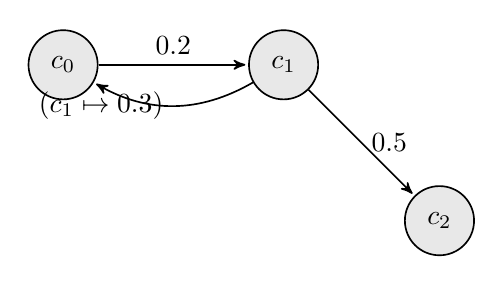
\begin{tikzpicture}[->,>=stealth',shorten >=1pt,auto,node distance=2.8cm,
                semithick]
        \tikzstyle{every state}=[fill={rgb:black,1;white,10}] 
        \node[state] (c0) {$c_0$};
        \node[state] (c1) [right of=c0] {$c_1$};
        \node[state] (c2) [below right of=c1] {$c_2$};

        \path (c0) edge  node [above] {0.2} (c1);
        \path (c1) edge  node [right] {0.5} (c2);
        \path (c1) edge [bend left] node [left] {$(c_1 \mapsto 0.3)$} (c0);
    \end{tikzpicture}
    \caption{An example of a graph that represents a stochastic compartmental model with 3 compartments. The label of the $(c_2, c_0)$ edge is a vector with $0.3$ indexed by $c_1$ and all other values are zero (thus omitted to avoid clutter).}
    \label{fig:stochastic_model}
\end{figure}

\end{document}